\documentclass{article}
\usepackage{graphicx}
\usepackage{wrapfig}
\usepackage{array}
\usepackage{url}
\usepackage{graphicx}
\usepackage{wrapfig}
\usepackage{float}
\title{Packet Analysis (Chapter4 Case Study)}

\author{Mohsen Tavakoli, Joseph Maan Anayee, Oluwaseyi Akinlade, Nima Moradianzadeh}

\begin{document}

\maketitle

\section{Problem description}
In this assignment we aims to analyzing the packet capture and also collect the information from a suspected persons activities.
 
The following questions will help guide your investigation:
• Provide any online aliases or addresses and corresponding account credentials that
may be used by the suspect under investigation.
• Who did Ann communicate with? Provide a list of email addresses and any other
identifying information.
• Extract any transcripts of Ann’s conversations and present them to investigators.
• If Ann transferred or received any files of interest, recover them.
• Are there any indications of Ann’s physical whereabouts? If so, provide supporting
evidence.
Network:
• Internal network: 192.168.30.0/24
• DMZ: 10.30.30.0/24
• The “Internet”: 172.30.1.0/24 [Note that for the purposes of this case study, we are
treating the 172.30.1.0/24 subnet as “the Internet.” In real life, this is a reserved nonreturnable
IP address space.]
Evidence: Investigators provide you with a packet capture from Ann’s home network,
“evidence-packet-analysis.pcap.” They also inform you that in the course of their monitoring,
they have found that Ann’s laptop has the MAC address 00:21:70:4D:4F:AE
\section{Experiment}
\subsection{simulation}
In order to emulate the network of the problem we used GNS3. GNS3 can be used in order to emulating the complex network. Virtual devices and actual devices can be set by this software\cite{amyot2014system}.



<<<<<<< HEAD
\subsection{Tools Used}
To conduct the experiment we mainly used two tools interacting together. The first tool we used to setup the network is GNS3 and the second tool we used is Wireshark to analyze the packets captured during normal network communication.


\subsubsection{GNS3 (Graphical Network Simulator-3)}
GNS3 is a network software emulator. It facilitates the simulation of network traffic using real and virtual devices. GNS3 was initially intended to simulate Cisco routers and switches but then it was expanded to support other platforms as well and today it is used emulate various complex networks.  GNS3 Was used in our experiment to setup and emulate network traffic. 


We are able to create routers and switches and add different computers on the network. Doing so, we were able to communicate with different computers across different switches \cite{hassine2014toward}.


\subsubsection{Wireshark}
Is a network tool that is used to analyze packets transmitted over a computer network. It is open source and supported across many platforms. The way it operates is very similar to TCPDUMP however it has a graphical user interface to make it easier for the network engineer to troubleshoot the network \cite{orebaugh2006wireshark}.


For the sake of our experiment, a capture tool is added between the two routers shown in network topology that captures traffic between two routers. The capture tool capture the network packets being transmitted over the network for wireshark in order for them to be analyzed.

=======

\subsection{Network Topology}

The emulated topology(Figure.\ref{fig:TPLGY}) consists:

\begin{itemize}
	
	\item Two Cisco c7200 Routers (R1 and R2)
	\item Five Cisco Ethernet Switches (SW1 to SW5)
	\item Seven Virtual Machines (PC1 to PC7)
	\item Two Microsoft Loopback Adaptor 
\end{itemize}

The PCs are connected to the switches which are connected to one of the Reouters fast ethernet Ports:


\begin{itemize}
	
	\item Sw1 is configured on R1 interface f1/0 and 192.168.30.0/24
	\item Sw2 is configured on R1 interface f2/0 and 172.30.1.0/24
	\item Sw4 is configured on R1 interface f3/0 and 1923.164.137.0/24
	\item Sw3 is configured on R2 interface f1/0 and 192.122.52.0/24
	\item Sw5 is configured on R2 interface f2/0 and 190.168.136.0.24/24
\end{itemize}

R1 and R2(Cisco c720 Routers) are connected together on the fast Ethernet port 0:10.30.30.254 and 10.30.30.253 respectively.The R1 is active router for Sw1 ,Sw2 and SW4 and R2 is active Router for S5 and Sw3. Additionally, the virtual machines use Dynamic Host Configuration Protocol(DHCP) in order get IP address. This Protocol can be used in order to set the IP host and its related configuration information.


\begin{figure}[H]
	\begin{center}
		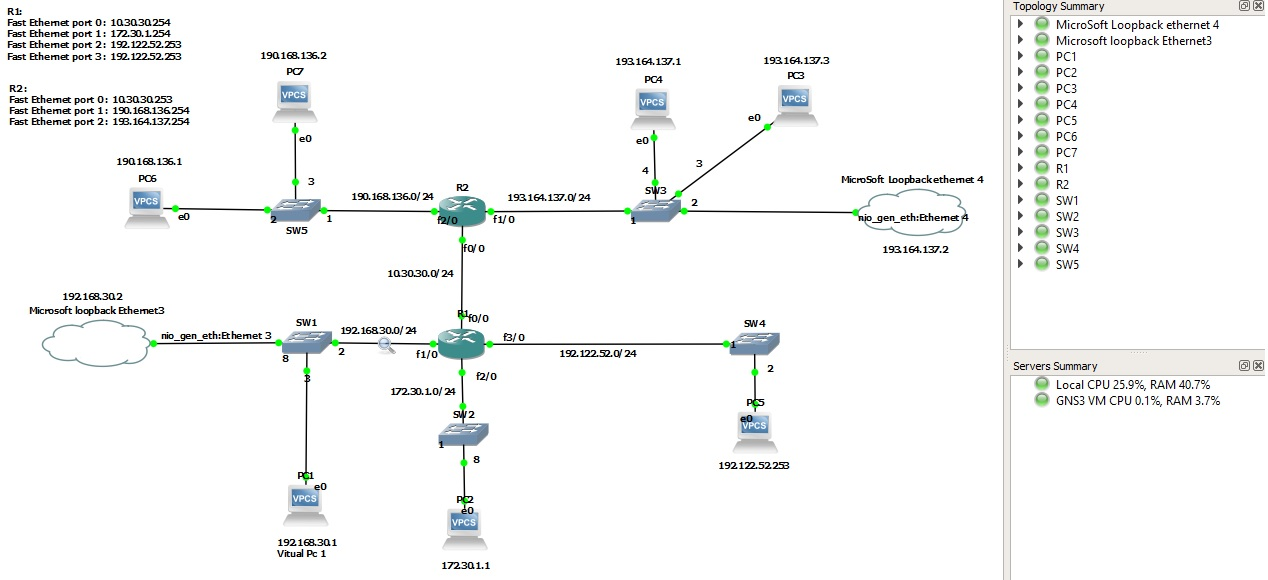
\includegraphics[width=0.6\textwidth]{Topology.jpg}
	\end{center}
	\caption{\small  Our Simulated Network Topology\newline}
	\label{fig:TPLGY}
\end{figure}
\subsection{Km-test Loopback}

Microsoft Loopback Adapter has some capabilities that can be used in our model. Firstly, it can be used for virtual network protecting by using Internet Connection Firewall. Secondly, Designer also can use it to share the files independently and design host-to-guest networking. Lastly, providing the Network Address Translation (NAT) and sharing connection to Internet are other capabilities of this software.\\
We installed MS Loopback as an additional Network adapter on the computer. In following, we described how we installed Microsoft Loopbaack Adapter:
In the Device Manager panel click on Action and choose the Add legacy Hardware. Now the installation page is opened (Figure.\ref{fig:KMINS}) . For more information about installation you can check this website:\\
	\url{https://technet.microsoft.com/en-us/library/cc708322(v=ws.10).aspx}


\begin{figure}[H]
	\centering
		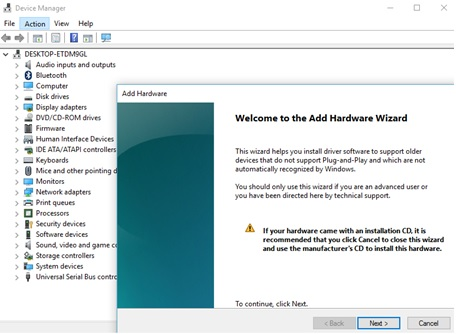
\includegraphics[width=0.48\textwidth]{LoopBackIns1.jpg}
	
	\caption{\small Microsoft KM-test Loopback Adapter Installation\newline}
	\label{fig:KMINS}
\end{figure}


NOTE: just note that you choose the Microsoft KM-TEST Loopback Adapter on the Network Adapters section (Figure.\ref{fig:KMINS2}) .


\begin{figure}[H]
	\begin{center}
		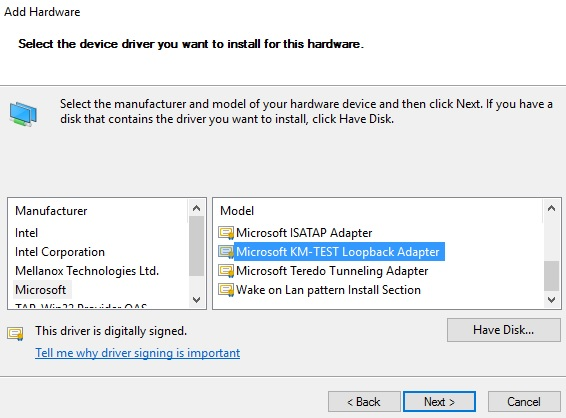
\includegraphics[width=0.48\textwidth]{LoopBackIns2.jpg}
	\end{center}
	\caption{\small Network Adapters section \newline}
	\label{fig:KMINS2}
\end{figure}


In Figure.\ref{fig:StatusEth}, you can see that there are two Real nodes configurations which are connected to the networks 193.164.137.0 and 192.168.30.0 in cloud figure.\\


These two LAN module in GNS3s simulated network are connected to a real PC and have different topologies for their connection. Figure.\ref{fig:StatusEth} shows that Ethernet 3 used the IP address 192.168.30.2 and Ethernet 4 using 172.30.1.2. Furthermore, both have same Gateway (255.255.255.0)


\begin{figure}[H]
	\begin{center}
		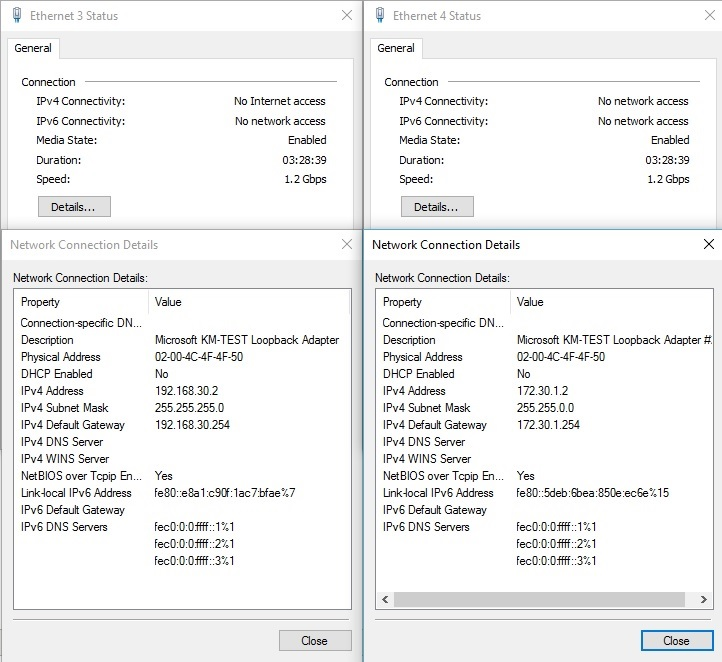
\includegraphics[width=0.48\textwidth]{Ethernet.jpg}
	\end{center}
	\caption{\small Ethernets Status \newline}
	\label{fig:StatusEth}
\end{figure}


Linux PCs:\\
Explain the Configuration here (contact me if you couldn’t)

\begin{figure}[H]
	\begin{center}
		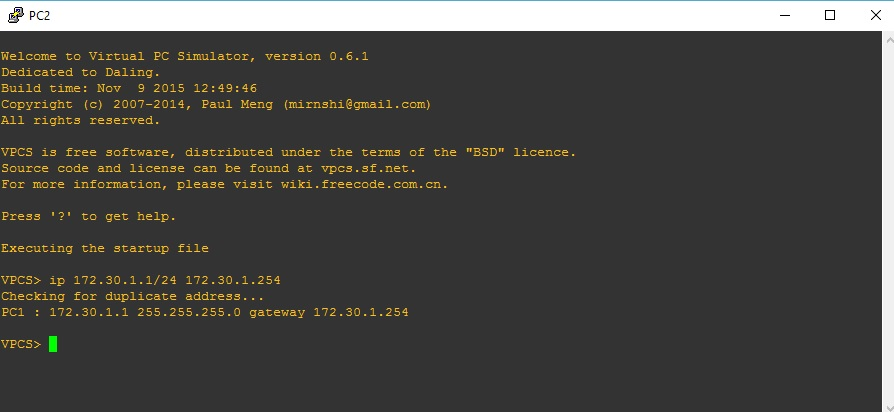
\includegraphics[width=0.48\textwidth]{VPC.jpg}
	\end{center}
	\caption{\small  \newline}
	\label{fig:VPC}
\end{figure}
Vpcs in Fig 5 is a virtual pc simulator found in GNS3, used for testing in GNS3 with ping and traceroute capabilities. Virtual pcs command : IP [address] [/mask] [gateway].The ip address of the virtual pc 2 is configured by entering the ip command then assigning 172.30.1.1/24 as the ip address and subnet then 172.30.1.254 as the gateway. The console then checks if it is a duplicate address and ping command is then used to test connectivity.

Ethernet Switches:\\
We configure the switches and grant access to all the ports for future computers.

\begin{figure}[H]
	\begin{center}
		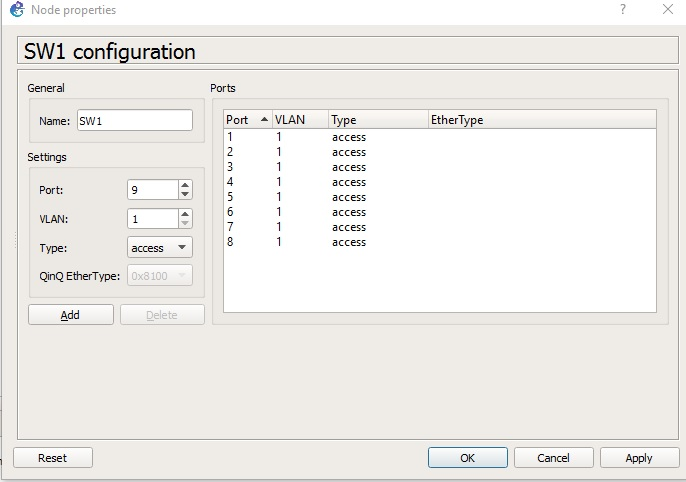
\includegraphics[width=0.48\textwidth]{Switchconf.jpg}
	\end{center}
	\caption{\small  \newline}
	\label{fig:Prd}
\end{figure}

\subsection{Routers configurations}

Figure.\ref{fig:Termconf} shows how an IP can be configured on a Cisco router interface. The first step, the router enabled to turn on privileged commands (If the password has been set for the router after entering enable the command line asked you to enter the password). Secondly, The second command (configure terminal) is used to enter to global configuration mode. Then you need to enter to the fast Ethernet Interface configuration mode, and the IP address and Gateway will be written in the next step. By default, the interface is "Administratively Down" means that the port is closed. So lastly, we used "no shutdown" command to enable it.

\begin{figure}[H]
	\begin{center}
		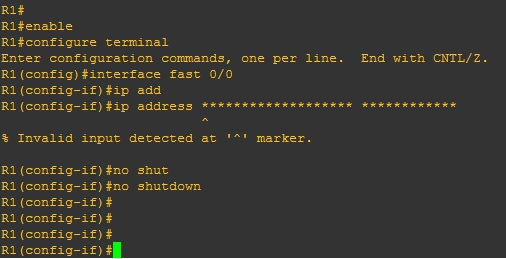
\includegraphics[width=0.48\textwidth]{Terminalconf.jpg}
	\end{center}
	\caption{\small Enter An IP to the Cisco Router \newline}
	\label{fig:Termconf}
\end{figure}

We configure each Router Interface.\\

Router RIP Configuration:

\begin{figure}[H]
	\begin{center}
		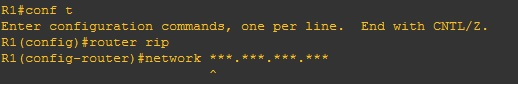
\includegraphics[width=0.48\textwidth]{RouterRip.jpg}
	\end{center}
	\caption{\small  \newline}
	\label{fig:Prd}
\end{figure}
Routing information Protocol (Rip): Fig 8 displays the routing Information Protocol. The Rip uses hop counts as a metric to determine the best path to a network and also prevents routing loops. The "router configuration terminal" command is first entered to start the rip process, then the "router rip" command is entered in the console, The "network *.*.*.*.*.*.*.*.*.*" command is used to assign networks that would participate in the rip process. The "show ip rip database" command displays all the networks in the RIP database. The "show ip protocols" displays the global configurations of the Rip process which include timers, network etc.

Router 1 Configuration: (do the exact thing for the ot

\begin{figure}[H]
	\begin{center}
		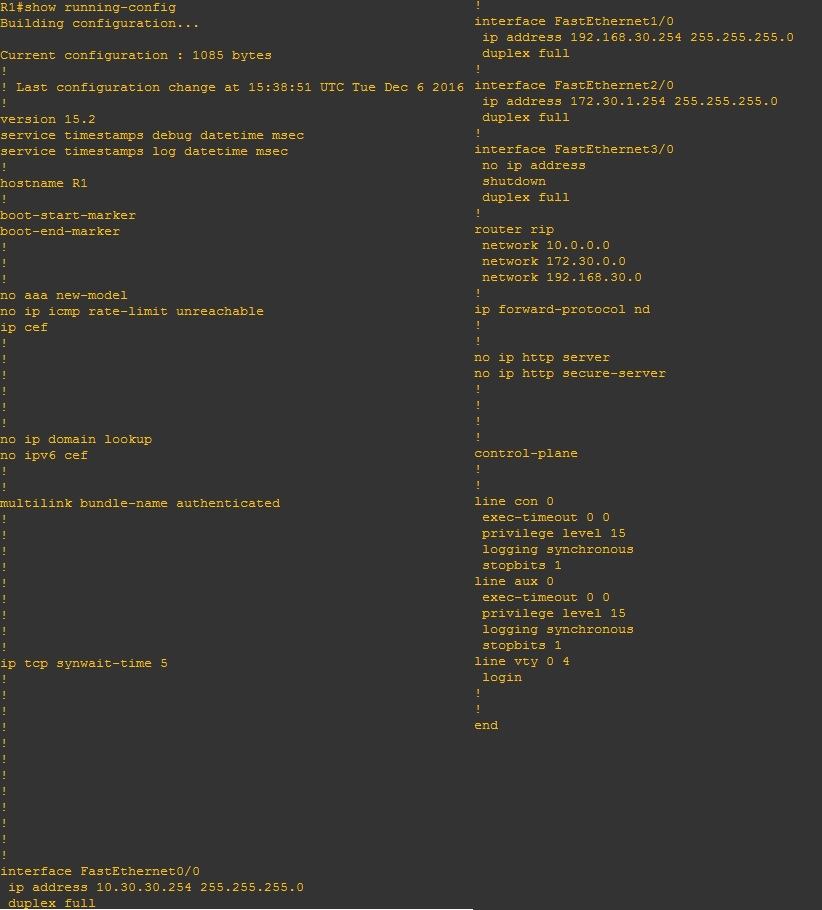
\includegraphics[width=0.48\textwidth]{Routerconfig.jpg}
	\end{center}
	\caption{\small  \newline}
	\label{fig:Prd}
\end{figure}


Wireshark:\\
When computers are communicating over the network, we used Wireshark to capcture the packets being sent back and forth. As shown in Figure 10 below list of packets captured, each packet holds significant of information, for example the sender and receiver. Each packet is stamped with time captured, source of the sender in ipv4 address format and destination address also in ipv4 along with the sending protocol. From the list pange, we are able to click on any packet and find more details about it in the tree view or byte view panes. 

\begin{figure}[H]
	\begin{center}
		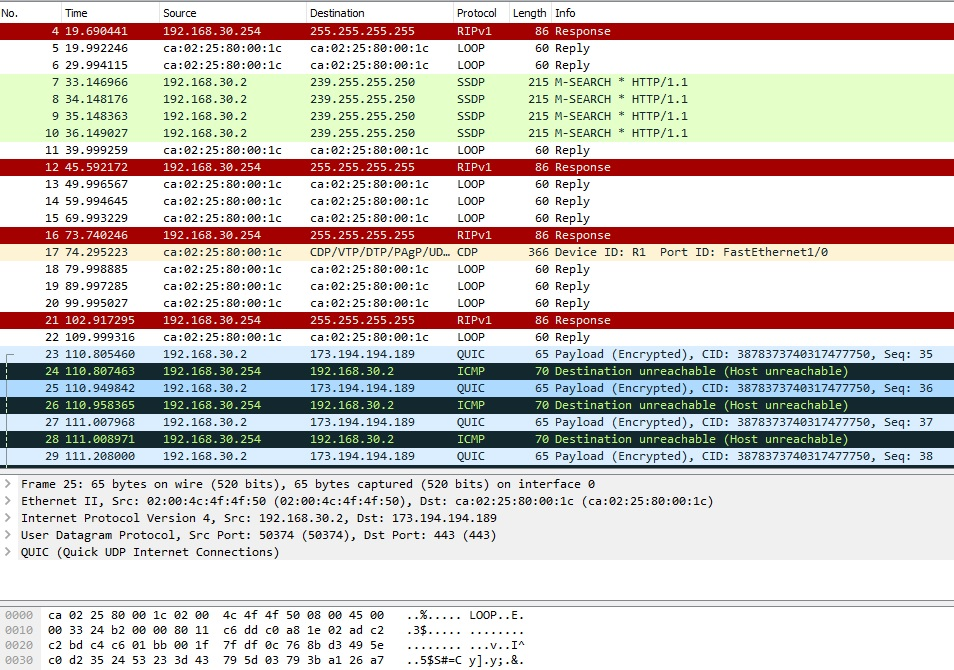
\includegraphics[width=0.48\textwidth]{wireshark.jpg}
	\end{center}
	\caption{Packets captured by Wireshark}
	\label{fig:Prd}
\end{figure}

Protocol Hierarchy:\\
Explain here….


\begin{figure}[H]
	\begin{center}
		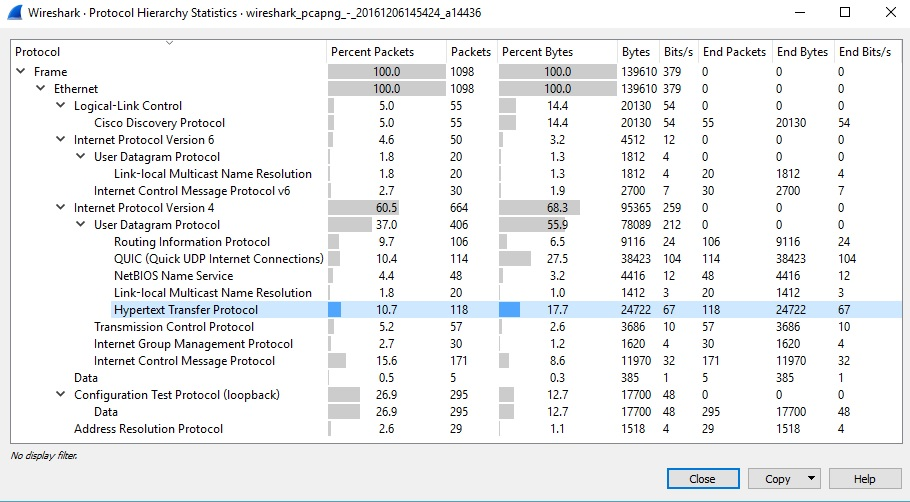
\includegraphics[width=0.48\textwidth]{Hierarchyst.jpg}
	\end{center}
	\caption{\small  \newline}
	\label{fig:Prd}
\end{figure}

\bibliographystyle{ieeetr}
\bibliography{Kent-Case-Study1}
\end{document}
